\documentclass{article}
\usepackage{blindtext}
\usepackage[T1]{fontenc}
\usepackage[utf8]{inputenc}
\usepackage{listings}
\usepackage{comment}
\usepackage{hyperref}

\hypersetup{
    colorlinks=true,
    linkcolor=blue,
    filecolor=magenta,
    urlcolor=cyan
}

\title{Recomendação de posts do blog Nerds Viajantes para conteúdo encontrado na web}
\author{Helder Ribeiro}
\date{\today}

\begin{document}

\maketitle

\pagebreak

\tableofcontents{}

\section{Motivação}

Hoje em dia a geração de conteúdo acontece de forma muito rápida. Acompanhar tudo que é gerado de forma manual é impraticável, senão impossível, e é
preciso automatizar determinadas tarefas. Uma das áreas onde a automatização pode ser feita é no processamento de textos e diversas informações podem ser 
extraídos dos textos que são escritos e compartilhados na internet, assim como em mídias privadas também.

Uma área que se destaca neste contexto é o processamento de linguagem natural (PLN), que consiste em um conjunto de técnicas que aplicadas a textos
permitem que diversas tarefas sejam executadas sobre esses textos. Uma destas tarefas é processar este conteúdo e identificar contextos dentro dele, 
permitindo que possamos levantar algumas informações como tópicos que relacionam estes documentos. A identificação deste contexto pode não ser simples
porque a mesma informação pode ser escrita de formas distintas utilizando linguagem natural.

\begin{itemize}
    \item velocidade de geração de conteúdo - Ok
    \item Geração de tráfego
    \item time to market
    \item sugestão de conteúdo para enriquecer textos
    \item sugestão de novas leiturs
    \item encontrar cópia do próprio
\end{itemize}

Natural language is messy, ambiguous and full of subjective interpretation, and sometimes trying to cleanse ambiguity reduces the language to an 
unnatural form.

\section{Algoritmo e estruturas de dados}

\subsection{Fonte de dados}
Durante a implementação do projeto, um objetivo foi manter a rotina principal (treinamento, cálculo de probabilidade dos tópicos e semelhança entre documentos) independente dos dados de treinamento e também dos dados de teste. O motivo disto é tirar o acoplamento da estrutura dos dados, do conteúdo e da forma como é feita a coleta.

Para isto foi proposta uma estrutura de dados onde foi definido o conceito de fonte de dados, que faz com que qualquer origem de dados escolhida pudesse ser trabalhada sem mudança no código fonte do algoritmo de recomendação.

Uma fonte de dados é uma abstração que tem como funcionalidade carregar os documentos de algum lugar e disponibilizar para o algoritmo de treinamento. Para ficar genérico foi criada a classe \textit{FonteDados} contendo o contrato de uma fonte, ou seja, quais métodos uma classe concreta precisa ter para fornecer os dados que o algoritmo precisa para o treinamento e também para montar o resultado com a semelhança entre os textos.

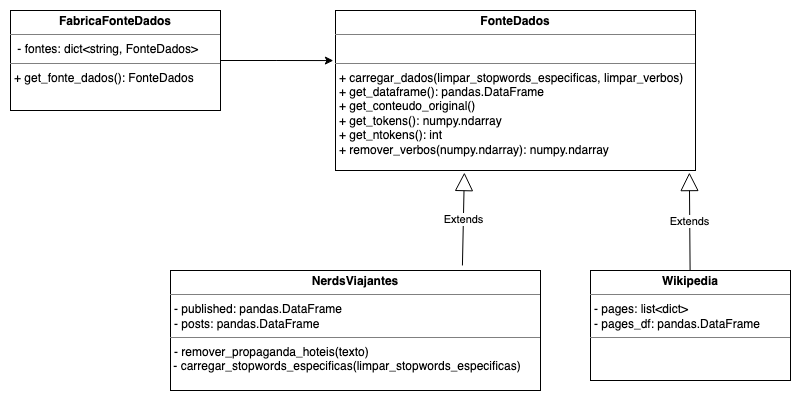
\includegraphics[scale=0.5]{fonte_dados.png}

Cada fonte de dados específica deve internamente carregar os dados e manter uma estrutura interna de forma a fornecer os documentos quebrados por tokens (palavras), assim como fornecer também um DataFrame contendo os seguintes dados:

\begin{itemize}
    \item id\_documento: id do documento na fonte de dados
    \item nome: nome do documento na fonte de dados
    \item titulo: titulo descritivo do documento na fonte de dados
    \item documento: conteudo original do documento
    \item n\_characters: tamanho do documento em caracteres
    \item tokens: tokens do documento apos limpeza
    \item n\_tokens: tamanho do documento em tokens
\end{itemize}

Desta forma as fontes de dados fornecem os dados de forma semelhante e podemos trabalhar com qualquer mídia e o algoritmo de recomendação não precisa ser alterado.
Para trabalhar com uma nova fonte de dados bastaria implementar uma subclasse de \textit{FonteDados} e implementar a parte específica que carrega os dados, faz limpeza e retorna os tokens e o DataFrame com os dados dos documentos.

\subsection{Treinamento LDA}

O módulo de treinamento LDA é responsável por ajustar um modelo para determinação de tópicos para os documentos de um conjunto de textos, assim como as 
palavras que mais contribuem para a formação de cada tópico. Recebe como parâmetros os documentos, o número de tópicos a serem escolhidos, 
além dos parâmetros do LDA passes, alpha e eta já explicados na seção de treinamento.

O treinamento consiste nos seguintes passos:

\begin{enumerate}
    \item Criar um dicionário com o conjunto total de palavras de todos os documentos. Este dicionário contém um mapeamento de um id interno para cada palavra
    \item Com base no dicionário, cria um \textit{corpus}, que é um mapeamento de frequência de ocorrência de cada palavra no conjunto inteiro de textos
    \item Faz o treinamento do modelo usando a classe \textit{LdaModel} do pacote \textit{gensim}
    \item Retorna como resultado do treinamento uma tupla com três elementos:
    \begin{itemize}
        \item Dicionário de palavras
        \item \textit{corpus}
        \item Resultado do modelo treinado
    \end{itemize}
\end{enumerate}

Segue o fragmento de código que faz este trabalho de treinamento:
\vspace{3mm} %3mm vertical space

\begin{lstlisting}[language=Python, style=mystyle, frame=lines, caption=Código fonte: Treinamento de modelo usando LDA]
    def ajustar_modelo(self, documentos, alpha=1e-2, eta=0.5e-2):
        # Cria dicionario
        id2word = dicionario.criar(documentos)

        # Cria corpus com base nos documentos e no mapeamento de id para palavra
        # Para cada documento faz a contagem de vezes que um determinado topico
        # aparece no documento
        corpus = [id2word.doc2bow(documento) for documento in documentos]

        print(f'Ajustando modelo com {self.num_topics} topicos e {self.passes} passes')

        # Treina modelo LDA        
        lda = LdaModel(corpus=corpus, id2word=id2word, 
                num_topics=self.num_topics, passes=self.passes, 
                alpha=alpha, eta=eta,
                random_state=0)

        return ResultadoTreinamentoLda(id2word, corpus, lda)
\end{lstlisting}

Para referência, um link do \href{https://github.com/heldergr/tcc-pucmg-2/blob/main/src/python/notebooks/treinamento/treinamento_lda.py}{código fonte do módulo de treinamento}.

\subsection{Cálculo de semelhança}

\subsection{Executor}

Foi criado um módulo executor para que pudessem ser variados os parâmetros de ajustes do modelo e gerar resultados para cada conjunto gerado por esta variação, permitindo uma comparação posterior dos resultados obtidos.
Este módulo recebe como parâmetro uma lista de cenários de testes. Cada cenário contém as informações:
\begin{itemize}
    \item fonte de dados de origem
    \item fonte de dados de destino
    \item topics
    \item alpha
    \item eta
    \item passes
\end{itemize}

Para cada combinação destes valores é feito o ajuste de modelo para os documentos de origem e o cálculo do documento de destino mais semelhante de 
cada documento de origem com base nas probabilidades que o documento contenha cada tópico.

\begin{comment}
    \lstinputlisting[language=Python, style=mystyle, frame=lines, caption=Código fonte: Cálculo de coerência de tópicos]{"/home/helder/estudos/tcc-pucmg-2/src/python/notebooks/main/executor.py"}
\end{comment}

Para referência, um link do \href{https://github.com/heldergr/tcc-pucmg-2/blob/main/src/python/notebooks/main/executor.py}{código fonte do executor de treinamento}.

O resultado gerado é um DataFrame com as seguintes colunas:

\begin{itemize}
    \item id\_cenario: identificador do cenário de testes
    \item fonte\_origem: descrição da fonte de origem
    \item id\_documento\_origem: identificador do documento na fonte de origem
    \item titulo\_documento\_origem: título do documento na fonte de origem
    \item fonte\_destino: descrição da fonte de destino
    \item id\_documento\_destino: identificador do documento na fonte de destino que tem a menor distância para o da fonte de origem referenciado na coluna id\_documento\_origem
    \item titulo\_documento\_destino: título do documento na fonte de destino
    \item distancia\_destino: distância calculada entre o documento na fonte de origem e o docmento na fonte de destino
    \item num\_topics: número de tópicos utilizado no modelo ajustado
    \item passes: parâmetro passes do algoritmo LDA
    \item eta: parâmetro eta do algoritmo LDA
    \item alpha: parâmetro alpha do algoritmo LDA
\end{itemize}


\section{Coleta de dados}

Parte dedicada a documentação de coleta de dados para treinamento.

\subsection{Posts Nerds Viajantes}

Obtenção de posts do banco de dados do blog Nerds Viajantes.

\subsection{Wikipedia}

Obtenção de páginas da Wikipedia para treinamento.

\subsection{Verbos em língua portuguesa}

Como parte do trabalho eu precisei da lista de verbos em língua portuguesa para analisar o levantamento de tópicos em documentos após remoção de verbos, 
que no contexto deste trabalho poderiam ser pouco relevantes ou até mesmo atrapalhar na definição dos tópicos.

A lista de verbos foi recuperada fazendo webscraping do site \url{https://www.conjugacao.com.br/verbos-populares}. Foi utilizada o pacote requests do Python 
para fazer a requisição das páginas e o pacote Beautiful Soap para extrair o conteúdo do resultado html retornado.

O total de verbos contidos nesta página é de 5000 e para que fossem retornados todos foram necessárias 50 requisições (são 100 verbos em cada página), 
uma para cada página de conteúdo no site.

Os verbos são gravados localmente em uma collection do MongoDB para que possam ser utilizados mais de uma vez sem necessidade de download a cada execução.
Cada documento gravado no MongoDB tem dois campos, o verbo original e o verbo \textit{stemmed}, conforme exemplo abaixo para o verbo \textit{falar}.

\begin{lstlisting}
    {
        'verbo': 'falar',
        'verbo_stemmed': 'fal'
    }
\end{lstlisting}

\begin{comment}
\subsection{Melhores Destinos}

Obtenção de posts com conteúdo de promoções do blog Melhores Destinos.    
\end{comment}


\section{Análise e Exploração dos Dados}

Antes de fazer qualquer trabalho de treinamento dos dados é preciso conhecer os dados em que estamos trabalhando. No contexto deste trabalho
duas coisas muito importantes a se compreender são os tamanhos dos documentos a serem trabalhados e o conjunto de palavras que fazem
parte do dicionário completo. As análises feitas demonstradas a seguir foram feitas na fonte de dados de posts do blog pois esta foi 
usada para criar o dicionário e fazer o treinamento do modelo.

\subimport{./}{analise_tamanho_documentos.tex}

\subimport{./}{analise_palavras_fontes_dados.tex}

\section{Processamento/Tratamento de Dados}

Nem sempre utilizamos o texto inteiro quando queremos extrair conhecimento do seu conteúdo, que no nosso caso significa encontrar tópicos com suas palavras e 
encontrar documentos em que estes tópicos estão presentes. Muitas palavras não são interessantes, como por exemplo aquelas que não agregam valor 
mas influenciam o treinamento de modelos, como as conhecidas \textit{stopwords}. Estas podem, inclusive, atrapalhar o processo de aprendizado 
ao adicionar ruído ao conjunto de dados e aumentar o custo computacional e o tempo de execução.

A limpeza de texto consiste então em remover dos nossos documentos originais este conjunto de palavras que não somente não agregam ao treinamento como atrapalham 
o seu funcionamento adequado. Parte das tarefas de limpeza é comum a todas as fontes de dados e parte é específica por fonte de dados escolhida.

Estas atividades são na essência uma tentativa de conversão de linguagem de texto para algo mais próximo do que o computador consegue entender melhor,
preparando os dados de textos para o processamento de linguagem natural.

\subsection{Limpeza comum}

Algumas tarefas de limpeza de texto são úteis e devem ser empregadas a qualquer fonte de dados, mesmo que com parâmetros diferentes.

\begin{itemize}
    \item Remoção de tags HTML: são apenas marcadores para definir a formatação de conteúdo html e não devem fazer parte dos dados de treinamento ou teste
    \item Remoção de pontuações: servem apenas para definir a estrutura do texto e não devem ser utilizados no treinamento
    \item Conversão para minúsculo: todo o conteúdo deve ser normalizado convertendo as letras para minúsculas de forma que palavras escritas com 
    \textit{case} diferente não sejam tratadas como entidades distintas
    \item Remoção de \textit{stopwords}: contempla a remoção de \textit{stopwords} gerais da linguagem dos textos, em nosso caso português. Esta lista é 
    obtida de um pacote de processamento de linguagem natural
    \item Remoção de palavras adicionais: remover do texto palavras que não são \textit{stopwords} mas atrapalham o treinamento de alguma forma. 
    É uma questão que deve ser avaliada especificamente para cada fonte de dados adicionais pois a lista é diferente em cada fonte de dados. Esta lista é obtida após análise de exploração e conhecimento da fonte de dados 
    \item \textit{Stemming}: redução de palavras para sua forma raiz, necessário para uma mesma palavra que seja escrita de formas distintas seja 
    tratada como apenas uma entidade. Além disso este tratamento diminui a dimensão do conjunto total de palavras e reduz custo computacional.
    Como exemplo podemos citar as palavras \textit{visitei} e \textit{visita} que seriam reduzidas a \textit{visit}
\end{itemize}

Para exemplificar a execução de limpeza de texto vamos usar a seguinte frase: 

\textit{"Após visitar a Lagoa Dourada nós decidimos voltar o hotel. Foi um dia muito bonito, esta foi uma das lagoas mais bonitas que já visitamos."}

Após a limpeza temos como resultado a seguinte lista de palavras: 

\textit{['após', 'visit', 'lago', 'dour', 'decid', 'volt', 'hotel', 'foi', 'dia', 'bonit', 'lago', 'bonit', 'visit']}

Importante perceber alguns alterações importantes em relação ao texto inicial:

\begin{itemize}
    \item Conversão da palavra \textit{Após} para \textit{após} com o \textit{a} minúsculo
    \item Remoção de \textit{stopwords} como \textit{a, nós, o, um, esta, uma, das, mais, que, já}
    \item Alteração de \textit{case} e conversão da palavra \textit{Lagoa}, desta forma as duas referências a \textit{lagoa} que estavam escritas de 
    forma diferente agora são tratados como uma mesma entidades
    \item Remoção de pontuações
\end{itemize}

\subsection{Posts Nerds Viajantes}

\subsubsection{Limpeza de palavras nos posts}

Além da limpeza de texto padrão, foi necessário eliminar outros conjuntos de palavras dos posts do blog. Após execução da análise dos tópicos nas primeiras 
execuções de treinamento do modelo foi identificado que alguns conjuntos de palavras não fazem sentido ser usados na definição do dicionário.

\begin{itemize}
    \item Remoção de \textit{caption}: A ferramenta \textit{Wordpress} utilizada uma notação específica para adicionar legendas às imagens, que não corresponde ao padrão html e por isto foi necessária uma limpeza específica deste conteúdo
    \item Remoção de \textit{stopwords} específicas: Palavras que não fazem parte da lista de \textit{stopwords} da linguagem mas que mesmo assim 
    atrapalham no treinamento do modelo
    \begin{itemize}
        \item Exemplos: fot, fic, visit, fotograf, dia, algum, par, passei, bem, restaurant
        \item A lista completa destas palavras se encontra no arquivo \href{https://github.com/heldergr/tcc-pucmg-2/blob/main/src/python/notebooks/data/remocao_nerds_viajantes.txt}{remocao\_nerds\_viajantes.txt} no repositório do projeto.
    \end{itemize}
    \item Remoção de verbos: A ideia da comparação dos documentos foi mais direcionada a características dos locais visitados e decidi remover os verbos do texto pois estes contribuiam muito na composição dos tópicos
\end{itemize}

\subsubsection{Limpeza de posts inteiros}

Além da limpeza de palavras dentro dos posts, foi necessário também remover alguns posts do conjunto a ser utilizado no treinamento.

Nosso blog também tem um pouco de foco em fotografia e por muito tempo disponibilizamos \textbf{papéis de parede} de fotos que nós tiramos e gostamos. 
Para divulgar os papéis de parede escrevemos vários posts e estes não são interessantes para o propósito deste trabalho, por isso resolvi removê-los.
A remoção foi relativamente fácil, visto que todos os posts deste conjunto tem o atributo \textit{name} começando com o prefixo \textit{papel-de-parede}.

Outro critério para remoção de posts inteiros foi o \textbf{tamanho do documento em tokens}. Em várias referências sobre o algoritmo de identificação 
de tópicos LDA, é recomendado utilizar documentos cuja quantidade de tokens seja acima de 40 ou 50. Analisando os tamanhos posts do blog eu notei 
que 42 tokens seria um bom limite e este passou a ser o tamanho a partir do qual os documentos seriam usados no treinamento.

Além dos dois conjuntos acima eu também optei por analisar manual e visualmente o conjunto de posts para remover pontualmente alguns cujo conteúdo 
não seria interessante no treinamento. Páginas na ferramenta \textit{Wordpress} são consideradas posts e a página de contato, por exemplo, 
não interessa no nosso contexto. Posts com conteúdo publicitário também foram removidos. Posts com conteúdo de valor temporal (divulgação de um 
evento, por exemplo) que não tem mais valor atualmente também foram removidos. A lista completa pode ser consultada no 
\href{https://github.com/heldergr/tcc-pucmg-2/blob/main/src/python/notebooks/limpeza/limpeza_posts.py}{módulo de limpeza de posts}.

\subsection{Wikipedia}

No caso dos posts do blog a limpeza de tags html em posts é feita no carregamento dos dados antes do treinamento, mas no caso das páginas da 
Wikipedia eu resolvi fazer esta limpeza apenas uma vez e gravar em um atributo separado, aproveitando as facilidades do MongoDB para alteração 
na estrutura de documentos.

Ao fazer um teste com cerca de duas mil páginas o tempo para remover as tags foi mais de um minuto e como seria um trabalho a ser executado a 
cada treinamento eu achei melhor já fazer este processo previamente.

O campo utilizado como base para a limpeza foi o \textit{text}, que contém o conteúdo em html. Neste campo o conteúdo da página fica dentro de 
parágrafos (atributo html \textit{p}) e elementos pré-formatados (atributo html \textit{pre}).

Para cada texto eu utilizei o componente \textit{BeautifulSoup} do módulo \textit{bs4} para extrair todos os parágrafos e pré-formatados para, 
em seguida, gravá-los em um campo separada chamado \textit{text\_clean}, que foi usado no identificação de documentos semelhantes.

O código fonte completo pode ser encontrado no 
\href{https://github.com/heldergr/tcc-pucmg-2/blob/main/src/python/notebooks/limpeza/limpeza_posts.py}{módulo de limpeza da Wikipedia}.


\section{Download Wikipedia}

\subsection{Download de páginas}

Na wikipedia as categorias tem dois tipos de membros filhos: páginas e outras categorias.
A estratégia de donwload de páginas envolveu escolher as categorias desejadas e fazer donwload tanto das subcategorias quanto das páginas filhas.

ESCREVER SOBRE ESCOLHA DAS CATEGORIAS

\subsubsection{Problemas}

Primeiro problema

Árvore inteiro iria ficar muito grande
Uma mesma página foi baixada mais de uma vez já que era referenciada por mais de uma categoria. Teve caso em que a mesma página foi baixada 5 vezes pois era 
referenciada por 5 categorias diferentes. Isto fez com que o conteúdo fosse também baixado mais de uma vez. A estratégia utilizada para resolver este problema 
envolveu selecionar ids da páginas para download do conteúdo usando distinct e ao fazer o download marcar como pronto utilizando updatemany (inicialmente estava 
usando) updateone, o que fez com que o conteúdo da mesma página fosse feito download mais de uma vez.

\subsubsection{Solução definitiva}

Para corrigir o problema optamos por trabalhar utilizamos apenas o conjunto de dados que temos no MongoDB para evitar acessos extras à API da Wikipedia.

\begin{itemize}
    \item Renomear collection de pages errada de "pages" para "pages\_incorreto". Feito no mongo shell com commando (db.pages.renameCollection('pages\_incorreto'))
\end{itemize}

\begin{comment}
\section{Treinamento de modelo}

Treinamento de modelo para sugestão de posts para determinados conteúdos.

\subsection{LDA}

LDA é um algoritmo de aprendizagem não supervisionado que associa tópicos a documentos. Documentos são como textos e cada um pode conter mais de um tópico.
Tópicos são formados por palavras e uma mesma palavra pode fazer parte de mais de um tópico, ou seja, uma mesma palavra contribui para a formação de vários 
tópicos. Os tópicos são descobertos durante o treinamento do modelo mas a quantidade de tópicos deve ser especificada a priori.

Após o treinamento do modelo um documento tem uma distribuição discrete de tópicos e um tópico tem uma distribuição discreta de palavras. 

Como exemplo temos... COLOCAR AQUI EXEMPLO DE UM DOCUMENTO, SEUS TÓPICOS E AS PALAVRAS QUE COMPOEM O TÓPICO.

\begin{itemize}
    \item DÚVIDA: DEVO EXPLICAR COM MAIS DETALHES A IMPLEMENTAÇÃO DO LDA? ACREDITO QUE NÃO...
\end{itemize}

Há vários tipos de uso para o algoritmo LDA, como entender melhor o tipo de documento um determinado conjunto de palavras (notícias, artigo na wikipedia, 
negócios), quantificar as palavras mais usadas e mais importantes em um texto ou mesmo encontrar semelhanças e recomendações de documentos. 

Neste trabalho eu usei LDA para encontrar semalhança entre textos de acordo com os tópicos do modelo treinado e fazer recomendações com base em textos novos.

LDA não tem boa performance com documentos curtos, como tweets, por exemplo, pois ele infere parâmetros a partir da observação de palavras e se não há palavras
suficientes não há as condições necessárias para um bom aproveitamento.

LDA é um algoritmo que trabalha com modelos do tipo bag of words, ou seja, não há importância na ordem das palavras. Outros algoritmos funcionam bem com sentençãs
estruturadas.

\subsubsection{Hiperparâmetros}

\begin{itemize}
    \item $\alpha$: Um valor baixo indica que documentos contém poucos tópicos contribuindo para os mesmos
    \item $\eta$: Um valor baixo indica que tópicos contém poucas palavras contribuindo para os mesmos, enquanto em um valor alto pode haver maior sobreposição 
    de palavras entre tópicos diferentes
\end{itemize}
\end{comment}

\section{Semelhança entre documentos para textos desconhecidos}

Ao obter a distribuição de frequência de palavras em um novo texto o gensim apenas considera as palavras existentes no dicionário original que foram usadas para 
treinar o modelo, descartando aquelas que não existiam. Estas últimas não serão consideradas na distribuição de tópicos. Isto é um problema na definição dos tópicos
do novo texto mas importante para identificar semelhanças com os documentos originais.

Uma forma de mitigar o problema acima é tentar fazer com que os dados de treinamento sejam o mais abrangente possível.

\subsection{Cálculo de semelhança (Similarity query)}

Com base na distribuição de tópicos em um novo texto nós podemos calcular a semalhança dele com outros documentos, por exemplo aqueles usados no treinamento
do modelo. No caso deste trabalho será feita a comparação com os posts do blog Nerds Viajantes. Para o cálculo da semelhança nós usaremos uma métrica chamada
\textbf{distância Jensen-Shannon} para encontrar os documentos que apresentam maior semalhança.

Esta métrica determina o quão próximos estatisticamente falando dois documentos estão próximos, comparando a divergência entre a distribuição de tópicos
entre eles. Esta distância é simétrica, ou seja, a distância entre dois documentos A e B é a mesma de B e A, o que está de acordo com o propósito deste trabalho.

Para distribuições discretas P e Q, a \textbf{divergência Jensen-Shannon}, JSD, é definida como:

\[JSD(P||Q) = 1/2D(P||M) + 1/2D(Q||M)\]

onde \(M = 1/2(P + Q)\)

A raiz quadrada da \textbf{divergência Jensen-Shannon} é a \textbf{distância Jensen-Shannon}: \(\sqrt{JSD(P||Q)}\)

Quanto menor a \textbf{Jensen-Shannon distance} maior é a semelhança entre duas distrições, ou seja, maior a semelhança entre dois documentos.

Para encontrar os documentos mais semelhantes a um novo texto nós calculamos as probabilidades dos tópicos do novo texto e calculamos a 
\textbf{distância Jensen-Shannon} deste para os textos aos quais queremos comparar (usando as probabilidades dos tópicos deles) e ordenamos pelas 
menores distâncias para obter os mais semelhantes.

\section{Resultados}

Como foi a execução. Estratégia. Se não documentar aqui, colocar em outro lugar.
Mostrar as várias combinações de parâmetros.

\begin{itemize}
    \item Formato em que os resultados são gravados, estrutura do documento
    \begin{itemize}
        \item Quantos resultados foram gerados?
    \end{itemize}
    \item Pegar um pequeno conjunto de origem, analisar os recomendados e identificar tópicos e palavras que justifiquem a semelhança
    \item Estatísticas disparidade entre recomendados para documentos de origem (para cada documento, pegar quantos destinos distintos ele 
    referencia e fazer média e desvio padrão destes números)
    \item Gráfico de distâncias médias por número de tópicos
\end{itemize}

\subimport{./}{plano_execucao.tex}
\subimport{./}{comportamento_variacao_distancias.tex}
\subimport{./}{variabilidade_documentos_recomendados.tex}
\subimport{./}{topico_dominante.tex}    


\subsection{Tecnologias}

\begin{itemize}
    \item \textbf{Docker}: execução de ferramentas em containers com base em imagens das mesmas. Muito útil para evitar a complexidade de instalar softwares 
    localmente. Utilizada para execução de:
        \begin{itemize}
            \item MongoDB
            \item Mysql
        \end{itemize}
    \item \textbf{Git}: Versionamento do código fonte
    \item \textbf{Latex}: escrita de documentação e geração de relatório PDF
    \item \textbf{Python}: linguagem de programação utilizada para escrever todo o código deste trabalho, sendo escolhida a versão 3.8. Os principais pacotes que 
    utilizei estão listados abaixo (a lista completa pode ser encontrada no arquivo requirements.txt no repositório do projeto):
        \begin{itemize}
            \item bs4
            \item gensim
            \item matplotlib
            \item mysql
            \item nltk
            \item numpy
            \item pandas
            \item pymongo
            \item seaborn
            \item wordcloud
        \end{itemize}
    \item \textbf{Visual Studio Code}: IDE utilizada para escrever o código fonte 
\end{itemize}

\section{Links}

Aqui estão links para recursos que exibem o trabalho realizado.

\begin{itemize}
    \item Vídeo Youtube: \url{www.youtube.com}
    \item Repositório Git: \url{www.github.com/heldergr}
    \item Jupyter Notebooks
        \begin{itemize}
            \item Treinamento de modelo
            \item Análise palavras em documentos
            \item Análise de tópicos gerados no treinamento
            \item Cálculo de análise de valores de coerências
        \end{itemize}
\end{itemize}

\section{Referências}

\subsection{Artigos}

\begin{itemize}
    \item LDA and Document Similarity: \url{https://www.kaggle.com/ktattan/lda-and-document-similarity}
    \item Text Cleaning Methods for Natural Language Processing: \url{https://towardsdatascience.com/text-cleaning-methods-for-natural-language-processing-f2fc1796e8c7}
    \item Text Cleaning in Natural Language Processing(NLP): \url{https://medium.com/analytics-vidhya/text-cleaning-in-natural-language-processing-nlp-bea2c27035a6}
\end{itemize}

\subsection{Ferramentas e tecnologias}

\begin{itemize}
    \item Gensim LDA Model: \url{https://radimrehurek.com/gensim/models/ldamodel.html}
    \item Latex tutorial: \url{https://www.overleaf.com/learn/latex/Sections\_and\_chapters}
    \item Pyhton regex: \url{https://docs.python.org/3/library/re.html}
    \item Seaborn aesthetics: \url{http://seaborn.pydata.org/tutorial/aesthetics.html}
\end{itemize}

\end{document}
